%
% This is a borrowed LaTeX template file for lecture notes for CS267,
% Applications of Parallel Computing, UCBerkeley EECS Department.
% Now being used for CMU's 10725 Fall 2012 Optimization course
% taught by Geoff Gordon and Ryan Tibshirani.  When preparing
% LaTeX notes for this class, please use this template.
%
% To familiarize yourself with this template, the body contains
% some examples of its use.  Look them over.  Then you can
% run LaTeX on this file.  After you have LaTeXed this file then
% you can look over the result either by printing it out with
% dvips or using xdvi. "pdflatex template.tex" should also work.
%

\documentclass[UTF8,oneside]{article}

% \usepackage[UTF8,scheme=plain]{ctex}
\usepackage[AutoFakeBold,AutoFakeSlant,CJKecglue]{xeCJK}  % 载入 xeCJK以支持中文,支持伪粗体,伪斜体 , 去掉CJK 文字与西文字体间的空格
\usepackage[margin=1in]{geometry}
\usepackage{amsmath,amsthm,amssymb}
\usepackage{graphicx}
\usepackage{autobreak}
\usepackage{tikz}
\usepackage{array}
\usetikzlibrary{positioning} %为了实现相对位置的设定
\usepackage{xcolor} %为了实现不同的颜色
\setCJKmainfont{宋体}                                         % 设置中文中文字体
\setCJKmonofont{宋体}                                        % 设置中文等宽字体
% \setCJKsansfont{宋体}
% \setCJKmainfont{SimSun}[BoldFont=SimHei, ItalicFont=KaiTi]
\setlength{\oddsidemargin}{0.25 in}
\setlength{\evensidemargin}{-0.25 in}
\setlength{\topmargin}{-0.6 in}
\setlength{\textwidth}{6.5 in}
\setlength{\textheight}{8.5 in}
\setlength{\headsep}{0.75 in}
\setlength{\parindent}{0 in}
\setlength{\parskip}{0.1 in}

%
% ADD PACKAGES here:
%

\usepackage{amsmath,amsfonts,graphicx}

%
% The following commands set up the lecnum (lecture number)
% counter and make various numbering schemes work relative
% to the lecture number.
%
\newcounter{lecnum}
\renewcommand{\thepage}{\thelecnum-\arabic{page}}
\renewcommand{\thesection}{\thelecnum.\arabic{section}}
\renewcommand{\theequation}{\thelecnum.\arabic{equation}}
\renewcommand{\thefigure}{\thelecnum.\arabic{figure}}
\renewcommand{\thetable}{\thelecnum.\arabic{table}}

%
% The following macro is used to generate the header.
%
\newcommand{\lecture}[4]{
   \pagestyle{myheadings}
   \thispagestyle{plain}
   \newpage
   \setcounter{lecnum}{#1}
   \setcounter{page}{1}
   \noindent
   \begin{center}
   \framebox{
      \vbox{\vspace{2mm}
    \hbox to 6.28in { {\bf Fundamentals Of Information Science
	\hfill 2022 Spring} }
       \vspace{4mm}
       \hbox to 6.28in { {\Large \hfill   #2  \hfill} }
       \vspace{2mm}
       \hbox to 6.28in { {\it 学生: #3 \hfill 时间: #4} }
      \vspace{2mm}}
   }
   \end{center}
   \markboth{Lecture #1: #2}{Lecture #1: #2}

}
%
% Convention for citations is authors' initials followed by the year.
% For example, to cite a paper by Leighton and Maggs you would type
% \cite{LM89}, and to cite a paper by Strassen you would type \cite{S69}.
% (To avoid bibliography problems, for now we redefine the \cite command.)
% Also commands that create a suitable format for the reference list.
\renewcommand{\cite}[1]{[#1]}
\def\beginrefs{\begin{list}%
        {[\arabic{equation}]}{\usecounter{equation}
         \setlength{\leftmargin}{2.0truecm}\setlength{\labelsep}{0.4truecm}%
         \setlength{\labelwidth}{1.6truecm}}}
\def\endrefs{\end{list}}
\def\bibentry#1{\item[\hbox{[#1]}]}

%Use this command for a figure; it puts a figure in wherever you want it.
%usage: \fig{NUMBER}{SPACE-IN-INCHES}{CAPTION}
\newcommand{\fig}[3]{
			\vspace{#2}
			\begin{center}
			Figure \thelecnum.#1:~#3
			\end{center}
	}
% Use these for theorems, lemmas, proofs, etc.
\usepackage{amsthm}
\newtheorem*{Solution}{Solution}
\newtheorem{theorem}{Theorem}[lecnum]
\newtheorem{lemma}[theorem]{Lemma}

\newtheorem{proposition}[theorem]{Proposition}
\newtheorem{claim}[theorem]{Claim}
\newtheorem{corollary}[theorem]{Corollary}
\newtheorem{definition}[theorem]{Definition}
% \newenvironment{proof}{{\bf Proof:}}{\hfill\rule{2mm}{2mm}}

% **** IF YOU WANT TO DEFINE ADDITIONAL MACROS FOR YOURSELF, PUT THEM HERE:

\newcommand\E{\mathbb{E}}

\begin{document}
%FILL IN THE RIGHT INFO.
%\lecture{**LECTURE-NUMBER**}{**DATE**}{**LECTURER**}{**SCRIBE**}
\lecture{1}{Homework8}{华园(202000120027))}{2022.3.23}
%\footnotetext{These notes are partially based on those of Nigel Mansell.}

% **** YOUR NOTES GO HERE:

% Some general latex examples and examples making use of the
% macros follow.
%**** IN GENERAL, BE BRIEF. LONG SCRIBE NOTES, NO MATTER HOW WELL WRITTEN,
%**** ARE NEVER READ BY ANYBODY.

\section*{Problem 1.} % Don't be this informal in your notes!
Carl Coder implements a simple slotted Aloha-style MAC for his rooni's wireless network. His room has only two backlogged nodes, A and B. Carl picks a transmission probability of $2 p$ for node A and $p$ for node B. Each packet is one time slot long and all transmissions occur at the beginning of a time slot.\\
	(a) What is the utilization of Carl's network in terms of $p$ ?\\
(b) What value of $p$ maximizes the utilization of this network, and what is the maximum utilization?\\
(c) Suppose node $A$ and node $B$ can freely choose their transmission probabilities $p_{A}$ and $p_{B}$. How to choose $p_{A}$ and $p_{B}$ such that the throughput achieved by $\mathrm{A}$ is three times the throughput achieved by B and the utilization of his network is maximized.
\begin{Solution}
\end{Solution}
(a)\\
The probability that each time slot transmission is effective is:\\
\begin{align*}
P_{success}&=p(1-2p)+2p(1-p)\\
&=3p-4p^2
\end{align*}
Suppose there are N time slots,the utilization of Carl's network is:\\
\begin{align*}
U&=\frac{NP_{success}}{N}\\
&=3p-4p^2
\end{align*}

(b)\\
\begin{align*}
U&=3p-4p^2\\
\frac{dU}{dp}&=3-8p\\
let \frac{dU}{dp}=3-8p=0,we\,can\,&get\,that\,when\,p=\frac{3}{8},the\,utilization\,is\,max\\
p_0=\frac{3}{8}\qquad&\qquad U_{max}=\frac{9}{16}
\end{align*}
(c)\\
According to the meaning of the question, we can get:
\begin{align*}
P_A(1-P_B)&=3P_B(1-P_A)\\
P_B&=\frac{P_A}{3-2P_A}\\
\end{align*}
The utilization is:
\begin{align*}
U&=P_A+P_B-2P_AP_B\\
U&=\frac{4(P_A-P_A^2)}{3-2P_A}
\end{align*}
\begin{align*}
\frac{dU}{dp}=\frac{2P_A^2+6P_A-3}{(3-2P_A)^2}
\end{align*}
Let $\frac{dU}{dp}=0$,we can get:
\begin{align*}
P_A=\frac{3-\sqrt{3}}{2}\qquad P_B=\frac{\sqrt{3}-1}{2}
\end{align*}
At this time, utilization takes the maximum value:$$U_{max}=0.5359$$


\section*{Problem 2.}
Consider the the network shown in the following figure, Each node implementa Dijkstra's shortest paths algorithm using the link costs shown in the picture.\\
\begin{center}
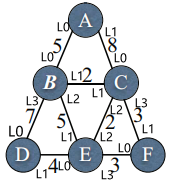
\includegraphics[scale=1.0]{a.png}
\end{center}
(a) Initially, node $D$ 's routing table contains only one entry, for itself. When $D$ runs Dijkstra's algorithm, in what order are nodes added to the routing table? List all possible answers.\\
(b) Now suppose the link cost for one of the links changes but all costs remain nonnegative. For each change in link cost listed below, state whether it is possible for the route at node $C$ (i.e., the link used by $C$ ) for any destination to change, and if so, name the destination(s) whose routes may change.\\
\begin{center}
i. The cost of link (B, D) increases:\\
ii. The cost of link (B, D) decreases:\\
iii. The cost of link (B, E) increases:\\
iv. The cost of link (B, E) decreases:
\end{center}
\begin{Solution}
\end{Solution}
\begin{table}[h]
\centering
\begin{tabular}{|c|c|c|c|c|c|c|c|c|c|c|c|c|c|c|}
\hline
Step& u &Nodeset &A &B &C &D &E &F &A &B &C &D &E &F \\
\hline
0 &  &[A,B,C,D,E,F] &$\infty$ &$\infty$ &$\infty$& 0 &$\infty$ &$\infty$ &? &? & ? & -- &? &?\\
\hline
1 & D &[A,B,C,E,F] &$\infty$ &7 &$\infty$& 0 &4 &$\infty$ &? &L0 & ? & -- &L1 &?\\
\hline
2 & E &[A,B,C,F] &$\infty$ &7 & 6 & 0 &4 &7 &? &L0 & L1 & -- &L1 &L1 \\
\hline
3 & C &[A,B,F] &14 &7 & 6 & 0 &4 &7 &L1 &L0 & L1 & -- &L1 &L1 \\
\hline
4 & B &[A,F] &12 &7 & 6 & 0 &4 &7  &L0 &L0 & L1 & -- &L1 &L1\\
\hline
5& F &[A]  &12 &7 & 6 & 0 &4 &7  &L0 &L0 & L1 & -- &L1 &L1 \\
\hline
6 & A &[]  &12 &7 & 6 & 0 &4 &7  &L0 &L0 & L1 & -- &L1 &L1\\
\hline
\end{tabular}
\label{TAB1}
\end{table}

\begin{table}[h]
\centering
\begin{tabular}{|c|c|c|c|c|c|c|c|c|c|c|c|c|c|c|}
\hline
Step& u &Nodeset &A &B &C &D &E &F &A &B &C &D &E &F \\
\hline
0 &  &[A,B,C,D,E,F] &$\infty$ &$\infty$ &$\infty$& 0 &$\infty$ &$\infty$ &? &? & ? & -- &? &?\\
\hline
1 & D &[A,B,C,E,F] &$\infty$ &7 &$\infty$& 0 &4 &$\infty$ &? &L0 & ? & -- &L1 &?\\
\hline
2 & E &[A,B,C,F] &$\infty$ &7 & 6 & 0 &4 &7 &? &L0 & L1 & -- &L1 &L1 \\
\hline
3 & C &[A,B,F] &14 &7 & 6 & 0 &4 &7 &L1 &L0 & L1 & -- &L1 &L1 \\
\hline
4 & F &[A,B] &14 &7 & 6 & 0 &4 &7 &L1 &L0 & L1 & -- &L1 &L1 \\
\hline
5& B &[A]  &12 &7 & 6 & 0 &4 &7	 &L0 &L0 & L1 & -- &L1 &L1 \\
\hline
6 & A &[]  &12 &7 & 6 & 0 &4 &7&L0 &L0 & L1 & -- &L1 &L1 \\
\hline
\end{tabular}
\label{TAB1}
\end{table}
we can get two possibilities:
\begin{center}
(1)DECBFA\\
(2)DECFBA
\end{center}
(b)\\
(i)if the cost of link(B,D)increases,the routes for C remain unchanged.\\
(ii)if the cost of link(B,D)decreases,When it decreases to less than 4, the shortest path from C to D changes from CED to CBD,so the routes for C changed\\
(iii)if the cost of link (B,E)increases,the route for C remain unchanged\\
(iv)if the cost of link (B,E)decreases,when it decrease to zero,the route CBED and CED have the same cost,so the route for C may change.


\section*{Problem 3.}
Consider the the network in Problem 2. If the network implements the distance-vector protocol, describe how the routing table at node $D$ changes after each step of integration. Given the network topology, how many steps are sufficient for the distance-vector protocol to converge (i.e., every node can find the shortest paths to its destinations).
\begin{Solution}
\end{Solution}
Round 1:
\begin{center}
{'D':(None,0)}
\end{center}
Round 2:
\begin{center}
{'B':('L0;,7)\\
'D':(None,0)\\
'E':('L1',4)}
\end{center}
Round 3:
\begin{center}
{'A':(L0,12)\\
'B':('L0,7)\\
'C':('L1',6)\\
'D':(None,0)\\
'E':('L1',4)\\
'F':('L1',7)}
\end{center}
we can get at Round 3,Node D find the shortest path,but for Node E,it doesn't find the shortest paths.for E:
Round 1:
\begin{center}
{'E':(None,0)}
\end{center}
Round 2:
\begin{center}
{'B':('L1,5)\\
'C':('L2',2)\\
'D':('L0',4)\\
'E':(None,0)\\
'F':('L3',3)}
\end{center}
Round 3:
\begin{center}
{'A':(L2,10)\\
'B':('L2,4)\\
'C':('L2',2)\\
'D':('L0',4)\\
'E':(None,0)\\
'F':('L3',3)}
\end{center}
Round 4:
\begin{center}
{'A':(L2,9)\\
'B':('L2,4)\\
'C':('L2',2)\\
'D':('L0',4)\\
'E':(None,0)\\
'F':('L3',3)}
\end{center}
so Node E need 4 steps to find the shortest paths,the distance-vector protocol to converge need 4 steps.
\section*{Problem 4.}
Annette Werker conducts tests between a server and a client using the sliding window protocol described in this chapter. There is no other traffic on the path and no packet loss. Annette finds that:\\
(1) With a window size $W_{1}=50$ packets, the throughput is 200 packets per second.\\
(2) With a window size $W_{2}=100$ packets, the throughput is 300 packets per second.\\
Annette finds that even this small amount of information allows her to calculate several things, assuming there is only one bottleneck link. Calculate the following:\\
(a) The minimum round-trip time between the client and server.\\
(b) The average queueing delay at the bottleneck when the window size is 100 packets.\\
(c) The average queue size when the window size is 100 packets.
\begin{Solution}
\end{Solution}
(a)The minimum round-trip time:
\begin{align*}
RTT_{min}&=W_1/200\\
&=0.25s
\end{align*}
(b,c)$$B·RTT_{min}=75$$
because $W_2>B·RTT_{min}$,we can get:$$W_2=B·RTT_{min}+Q$$ $$Q=25$$
According to Little's Law(i.e.Q=B·D), the average delay D at the bottleneck is:$$D=\frac{Q}{B}=\frac{1}{12}(seconds)$$

% **** THIS ENDS THE EXAMPLES. DON'T DELETE THE FOLLOWING LINE:

\end{document}





